\documentclass[sigconf]{acmart}

\usepackage{listings}
\usepackage{hyperref}
\usepackage{caption}
\usepackage{subcaption}
\usepackage{tikz}
\usetikzlibrary{arrows.meta}

\newcommand{\projectname}{\texttt{gingaf}}
\newcommand{\nclapp}{\texttt{ncl\_app}}
\newcommand{\htmlapp}{\texttt{html\_app}}

\copyrightyear{2026}
\acmYear{2026}
\setcopyright{cc}
\setcctype{by}
\acmConference[MM '26] {Proceedings of the 34th ACM International Conference on Multimedia}{November 10--14, 2026}{Rio de Janeiro, Brazil.}
\acmBooktitle{Proceedings of the 34th ACM International Conference on Multimedia (MM '26), November 10--14, 2026, Rio de Janeiro, Brazil}
\acmISBN{979-8-4007-2213-4/2026/11}
\acmDOI{10.1145/3767308.3834744}

\title{\projectname{}: Headless and Multiplatform Execution of ITU-SBTVD NCL Applications}

\author{Alan L.V. Guedes}
\orcid{0000-0003-0110-9975}
\affiliation{%
  \institution{Computer Science, University of Reading}
  \city{Reading}
  \country{UK}
}
\email{a.guedes@reading.ac.uk}
\renewcommand{\shortauthors}{Alan L. V. Guedes}

\begin{abstract}
The Nested Context Language (NCL) is a core component of the ITU-T and SBTVD television standards. It is legally mandated and installed on 100\% of certified Digital TV sets and set-top boxes across Brazil and several Latin American countries. This massive deployment impacts over 60 million people. However, the ecosystem of NCL development tools is limited. In this context, we present \projectname{}, an open-source implementation of an NCL player built in Flutter. It supports a headless execution engine that schedules NCL events in-memory without requiring any UI and provides a foundation for NCL developer tooling. We also propose a UI component that achieves multiplatform visual rendering of NCL documents on Windows, mobile, and Web from a single codebase.
\end{abstract}

\begin{CCSXML}
<ccs2012>
   <concept>
       <concept_id>10002951.10003227.10003251.10003256</concept_id>
       <concept_desc>Information systems~Multimedia content creation</concept_desc>
       <concept_significance>500</concept_significance>
       </concept>
 </ccs2012>
\end{CCSXML}

\ccsdesc[500]{Information systems~Multimedia content creation}

\keywords{TV, NCL, Ginga, Declarative Multimedia}

\settopmatter{printacmref=true}
\begin{document}

\maketitle

\section{Introduction}

The Nested Context Language (NCL) is a core component of the ITU-T~\cite{ITU_H761} and SBTVD~\cite{abnt_15606_2_2023} television standards. NCL defines a rich temporal and spatial synchronization model, allowing authors to specify how media objects interact over time using links and connectors. The NCL player is called Ginga. Ginga implementations are legally mandated and installed on 100\% of certified Digital TV sets and set-top boxes sold in Brazil and several other Latin American countries using the ISDB-T international television standard. Because it is legally mandated by local telecommunications entities (such as the SBTVD in Brazil), every major manufacturer (including Samsung, LG, Sony, and TCL) must include it directly into their television hardware. This wide adoption results in over 60 million people impacted. Given this reachability, NCL is also used by the government, e.g., Brazil4D~\cite{castro2016brazil} app targets low-income families to access public services, health information, and educational content. Recently, the application coding specification for the next-generation Brazilian digital television standard (aka, TV 3.0) has continued to advance the use of NCL~\cite{santos2026overview}.

Despite the above context, NCL developers and researchers still face two main development barriers. \textbf{P1) Lack of Accessible NCL Development Environment}: Traditional NCL players, such as the reference PUC-Rio C++ Ginga implementations, are tightly coupled to specific platform architectures (targeted Linux-based digital TV receivers), some require specialized OS setups to compile and run. This creates a steep barrier to entry that contrasts sharply with the trend in modern programming ecosystems, where major languages provide instant web-based playgrounds: HTML is directly executable in any browser\footnote{\url{https://developer.mozilla.org/en-US/docs/Web/HTML/Reference/Elements/img}}, and even native compiled languages such as Go\footnote{\url{https://go.dev/play/}} offer zero-install online environments for immediate experimentation. \textbf{P2) Lack of NCL Debugging Features}: Current NCL players do not allow developers to pause execution to investigate intermediate states or run the synchronization engine headless (without the graphical user interface), making testing and debugging highly manual and time-consuming.

\projectname{} (see available software\footnote{https://github.com/ginga-org-br/gingaf/releases/tag/v0.1.0} and demonstrations \footnote{https://alanlivio.github.io/paper-mm26-gingaf/}) addresses these challenges by introducing a modern, decoupled, and portable implementation of the NCL ecosystem. Written in Dart and built on the Flutter framework, \projectname{} separates document execution logic from the UI presentation component, exposing a clean API between them. This decoupling yields two primary contributions:
\begin{itemize}
  \item \textbf{Multiplatform execution (targeting P1)}: by leveraging Flutter, \projectname{} offers portable presentation support across diverse operating systems (Windows, macOS, Linux, iOS, Android, and Web) from a single codebase, removing the specialized hardware and environment setup barriers.
  \item \textbf{Headless execution (targeting P2)}: by separating the document state machine from the NCL UI component, the execution engine allows developers to run without a UI, advance time deterministically via a virtual clock, and tick calls to inspect and debug NCL application states in memory.
\end{itemize}

The remaining sections are organized as follows: NCL background (which can be skipped by readers familiar with NCL); related work; \projectname{} architecture; results and reproducibility instructions; and final remarks.

\section{NCL Background}
\label{sec:background}

NCL acts as a glue language, defining temporal and spatial synchronization among diverse media assets and viewer interactions, without prescribing media content formats~\cite{soares_nested_2006_model}. A \texttt{<media>} element may be an image, video, audio, text, or even imperative (e.g., Lua, Java) and declarative (e.g., HTML, SMIL) objects. It is defined by its type, content location, and properties. Furthermore, a media object can define an explicit duration (\texttt{explicitDur}) or temporal segments via the \texttt{<area>} element. The \texttt{<link>} element defines temporal relationships between nodes. It has a set of conditions that need to be satisfied to trigger a set of actions. The conditions can test the occurrence or property changes of media nodes or their segments; actions change node occurrences (start, pause, resume, stop) and properties (set).

To demonstrate the structure of NCL applications, we use a sample application (\texttt{video.ncl}) presented in Listing~\ref{lst:ncl}. The presentation defines a primary video (\texttt{video}) in lines~\ref{line:video_start}--\ref{line:video_end}, a green background media (\texttt{green\_bg}) in lines~\ref{line:green_start}--\ref{line:green_end}, and a red background media (\texttt{red\_bg}) in lines~\ref{line:red_start}--\ref{line:red_end} with an explicit duration of 2 seconds. Temporal behavior is coordinated by link elements: link \texttt{l1} starts the green background when area \texttt{a1} of the video begins (at 2s), and link \texttt{l2} stops the green background and starts the red background when area \texttt{a1} ends (at 4s). The application ends when the \texttt{red\_bg} ends at 6s (explicitDur 2s) and the main video ends decoding at 7s (video content duration). Visual execution screenshots at these timestamps are shown in Figure~\ref{fig:web} and Figure~\ref{fig:windows}. Video demonstrations are also present online\footnote{\url{https://alanlivio.github.io/paper-gingaf-acm-mm26/}}.

\begin{lstlisting}[language=XML, escapeinside={(*}{*)}, caption={video.ncl source code}, basicstyle=\scriptsize\ttfamily, frame=single, breaklines=true, aboveskip=1mm, belowskip=1mm, captionpos=b, numbers=left, label={lst:ncl}]
<ncl>
  <body>
    <port id="init" component="video"/>
    <media id="video" src="https://flutter.github.io/assets-for-api-docs/assets/videos/butterfly.mp4">(*\label{line:video_start}*)
      <area id="a1" begin="2s" end="4s"/>
    </media>(*\label{line:video_end}*)
    <media id="green_bg">(*\label{line:green_start}*)
      <property name="background" value="green"/>
      <property name="bounds" value="0%,80%,20%,20%"/>
    </media>(*\label{line:green_end}*)
    <media id="red_bg">(*\label{line:red_start}*)
      <property name="background" value="red"/>
      <property name="bounds" value="80%,80%,20%,20%"/>
      <property name="explicitDur" value="2s"/>
    </media>(*\label{line:red_end}*)
    <link id="l1">
      <bind role="onBegin" component="video" interface="a1"/>
      <bind role="start" component="green_bg"/>
    </link>
    <link id="l2">
      <bind role="onEnd" component="video" interface="a1"/>
      <bind role="stop" component="green_bg"/>
      <bind role="start" component="red_bg"/>
    </link>
  </body>
</ncl>
\end{lstlisting}

\begin{figure}[ht]
  \centering
  \Description{Two screenshots showing the execution of video.ncl on Windows at clock times 2.00s and 4.00s.}
  \begin{subfigure}{0.48\linewidth}
    \centering
    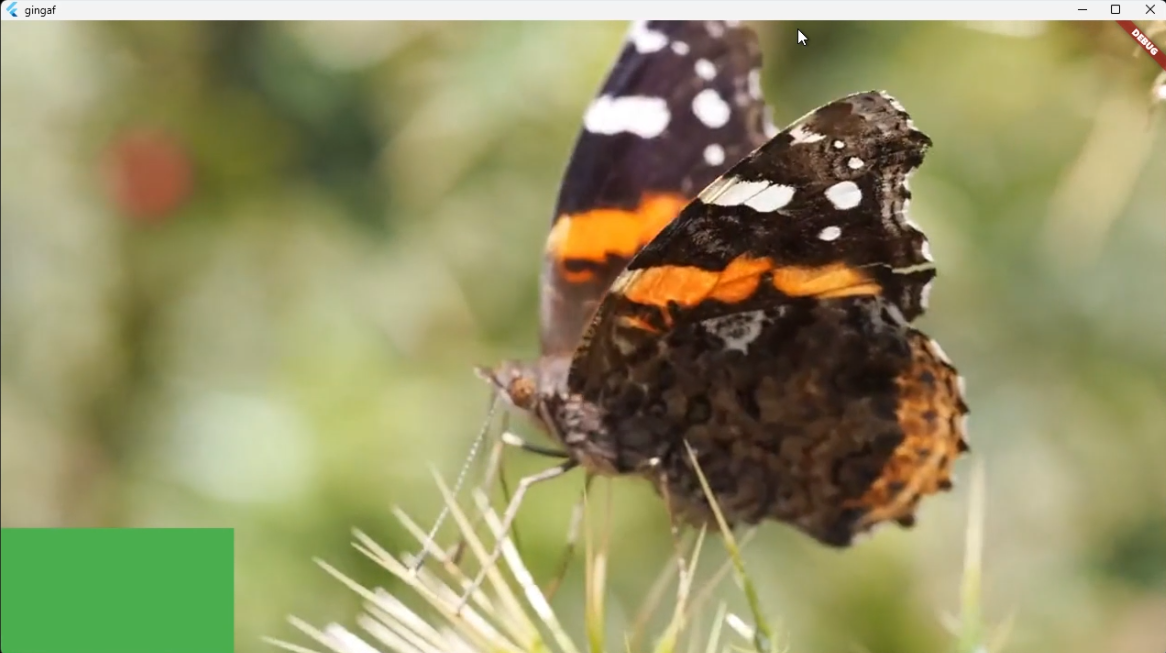
\includegraphics[width=\linewidth]{assets/app_clock2.png}
    \caption{Clock 2.00 (green\_bg starts).}
    \label{fig:web}
  \end{subfigure}%
  \hfill%
  \begin{subfigure}{0.48\linewidth}
    \centering
    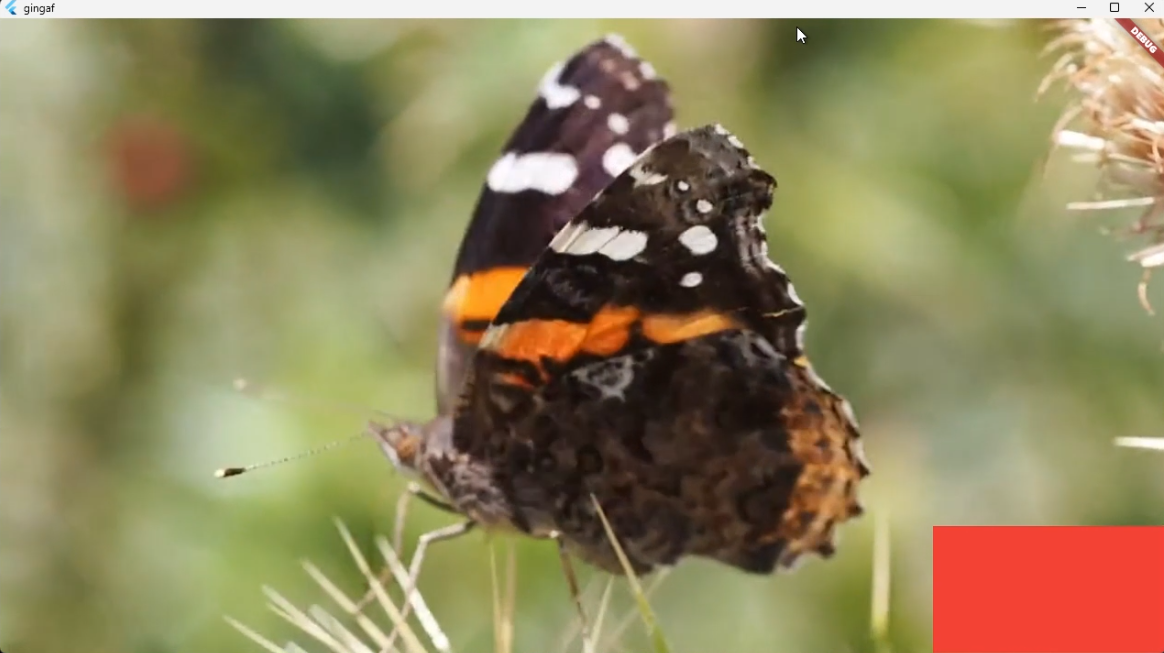
\includegraphics[width=\linewidth]{assets/app_clock4.png}
    \caption{Clock 4.00 (red\_bg starts).}
    \label{fig:windows}
  \end{subfigure}
  \caption{\texttt{video.ncl} execution (by \projectname{} on Windows).}
  \label{fig:running}
\end{figure}

Other advanced NCL features (not discussed for simplicity) include support for embedding scripts written in the lightweight scripting language Lua to implement complex interactive behavior, and a system of NCL editing commands that allows modifying applications on-the-fly. For example, in the application defined in Listing~\ref{lst:ncl}, the main \texttt{video} could represent a live TV streaming video, and the area \texttt{a1} could be dynamically inserted or updated on-the-fly by the broadcaster to indicate an advertisement.

\section{Related Work}

The development of NCL players has historically been led by the TeleMídia Lab at PUC-Rio\footnote{http://www.telemidia.puc-rio.br/}, producing several versions. We discuss the two main ones below.

\begin{figure}[t]
  \centering
  \Description{Communication diagram showing bidirectional coupling between NCL logic and NCL UI components in related work.}
  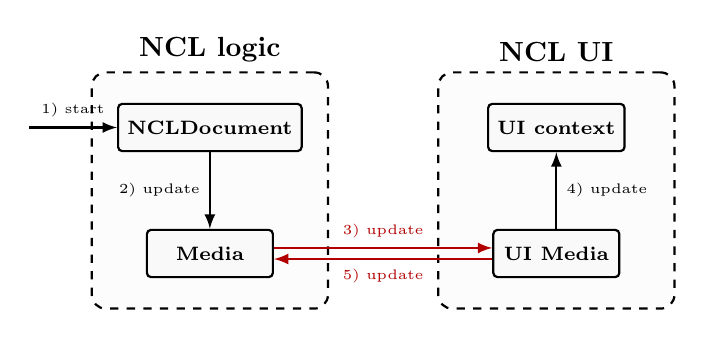
\begin{tikzpicture}[
      package/.style={draw, rectangle, rounded corners=5pt, minimum width=3.0cm, minimum height=3.0cm, fill=gray!2, dashed, thick, align=center},
      comp/.style={draw, rectangle, rounded corners=1.5pt, minimum width=1.6cm, minimum height=0.6cm, fill=gray!5, thick, align=center, font=\scriptsize},
      arrow/.style={-latex, thick},
      redarrow/.style={-latex, thick, color=red!70!black}
    ]
    \node[package] (doc_pkg) at (0, 0) {};
    \node[anchor=south] at (doc_pkg.north) {\textbf{NCL logic}};

    \node[package] (app_pkg) at (4.4, 0) {};
    \node[anchor=south] at (app_pkg.north) {\textbf{NCL UI}};

    \node[comp] (doc) at (0, 0.8) {\textbf{NCLDocument}};
    \node[comp] (media) at (0, -0.8) {\textbf{Media}};
    \node[comp] (ui) at (4.4, 0.8) {\textbf{UI context}};
    \node[comp] (ui_media) at (4.4, -0.8) {\textbf{UI Media}};

    \draw[arrow] (-2.3, 0.8) -- (doc.west) node[midway, above, font=\tiny] {1) start};
    \draw[arrow] (doc) -- (media) node[midway, left, font=\tiny] {2) update};
    \draw[redarrow] ([yshift=2pt]media.east) -- ([yshift=2pt]ui_media.west) node[midway, above, font=\tiny] {3) update};
    \draw[arrow] (ui_media) -- (ui) node[midway, right, font=\tiny] {4) update};
    \draw[redarrow] ([yshift=-2pt]ui_media.west) -- ([yshift=-2pt]media.east) node[midway, below, font=\tiny] {5) update};
  \end{tikzpicture}
  \caption{Related work communication diagram}
  \label{fig:coupled}
\end{figure}

PUC-Rio Ginga v0.13.6~\cite{moreno2010conciliando}\footnote{https://github.com/TeleMidia/ginga/releases/tag/v0.13.6} was designed for resource-constrained early-generation digital TV receivers. It used SDL\footnote{\url{https://www.libsdl.org}} as the UI context for rendering graphics and managing window events, and FFmpeg\footnote{\url{https://ffmpeg.org}} for audio/video decoding. Its execution model relied on multiple threads and event listeners to handle asynchronous media playback: dedicated threads monitored AV decoder callbacks and posted events into the NCL engine, creating concurrency that was difficult to test deterministically.

PUC-Rio Ginga v1.0~\cite{dodsworth2018dynamic}\footnote{https://github.com/TeleMidia/ginga/releases/tag/v1.0} modernized the renderer by adopting GTK\footnote{\url{https://www.gtk.org}} as the UI context and GStreamer\footnote{\url{https://gstreamer.freedesktop.org}} as the AV decoding pipeline. A key architectural advance was the move to a mono-threaded model inspired by synchronous execution: rather than spawning per-media threads, the engine advances state through a central tick loop, reducing race conditions and improving predictability.

The above related work shares a common problem: both implementations focus on desktop environments and never had web support because of their strong library decoding dependencies. They are heavy, complex to build, and require platform-specific drivers for multimedia rendering. Figure~\ref{fig:coupled} provides a simplified communication diagram that abstracts away libraries, threads, and callbacks to make clear that the NCL logic and NCL UI were tightly coupled. In it, \texttt{Media} objects directly reference \texttt{UI Media} components (arrow 3) and \texttt{UI Media} calls back into \texttt{Media} to report playback events (arrow 5). The red arrows highlight the fundamental problem: this bidirectional coupling makes it impossible to instantiate or test the NCL execution engine without an active rendering environment, preventing headless execution and deterministic debugging.

In contrast, \projectname{} introduces the NCL logic component as a fully self-contained package with no dependency on the NCL UI component. The execution engine exposes a clean \texttt{tick()} API, allowing it to run in-memory without any graphical context, enabling high-speed unit testing and step-by-step debugging of NCL synchronization logic.

Figure~\ref{fig:arch} illustrates how \projectname{} resolves this coupling. Unlike the related work, \texttt{NCLDocument} has no knowledge of any UI component and never holds a reference to \texttt{NCLMediaState} or any rendering object. The communication is strictly unidirectional: only the NCL UI sends messages to \texttt{NCLDocument} (arrows 2 and 5, highlighted in green). The NCL logic simply updates its internal \texttt{Media} state, and the NCL UI reads it back on demand. This asymmetry is the key difference from Figure~\ref{fig:coupled}, where the coupling runs in both directions across the boundary.

\section{\projectname{}}

\projectname{} is built using Dart and the Flutter\footnote{\url{https://docs.flutter.dev/}} framework. Dart is a multiplatform-oriented language, while Flutter is a runtime that allows Dart applications to run on desktop, mobile, and web. At its core, Flutter is based on widgets with states\footnote{\url{https://api.flutter.dev/flutter/widgets/State-class.html}}. \projectname{} is built around two main components (Figure~\ref{fig:arch}): the NCL Logic, implemented entirely in Dart, acts as a self-contained execution engine that manages the NCL event state machine with no knowledge of any display context; and the NCL UI, implemented as a Flutter widget, drives the engine and maps its output to native platform widgets. We discuss the two components in the next sections.

\begin{figure}[th!]
  \centering
  \Description{Communication diagram showing unidirectional interaction between NCL UI and NCL logic in gingaf.}
  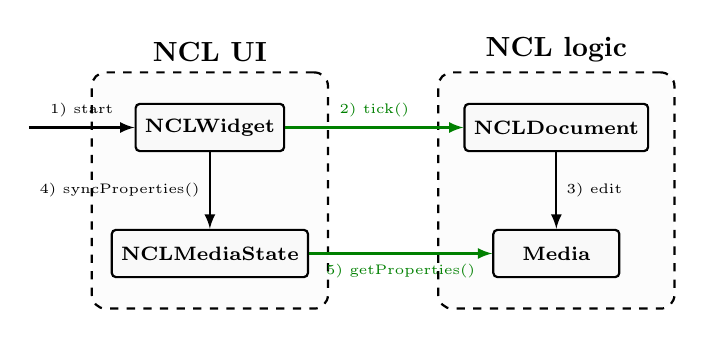
\begin{tikzpicture}[
      package/.style={draw, rectangle, rounded corners=5pt, minimum width=3.0cm, minimum height=3.0cm, fill=gray!2, dashed, thick, align=center},
      comp/.style={draw, rectangle, rounded corners=1.5pt, minimum width=1.6cm, minimum height=0.6cm, fill=gray!5, thick, align=center, font=\scriptsize},
      arrow/.style={-latex, thick},
      greenarrow/.style={-latex, thick, color=green!50!black}
    ]
    \node[package] (app_pkg) at (0, 0) {};
    \node[anchor=south] at (app_pkg.north) {\textbf{NCL UI}};

    \node[comp] (ncl_widget) at (0, 0.8) {\textbf{NCLWidget}};
    \node[comp] (widgets) at (0, -0.8) {\textbf{NCLMediaState}};

    \node[package] (doc_pkg) at (4.4, 0) {};
    \node[anchor=south] at (doc_pkg.north) {\textbf{NCL logic}};

    \node[comp] (ncl_doc_class) at (4.4, 0.8) {\textbf{NCLDocument}};
    \node[comp] (ncl_elements) at (4.4, -0.8) {\textbf{Media}};

    \draw[arrow] (-2.3, 0.8) -- (ncl_widget.west) node[midway, above, font=\tiny] {1) start};
    \draw[greenarrow] (ncl_widget) -- (ncl_doc_class) node[midway, above, font=\tiny] {2) tick()};
    \draw[arrow] (ncl_doc_class) -- (ncl_elements) node[midway, right, font=\tiny] {3) edit};
    \draw[arrow] (ncl_widget) -- (widgets) node[midway, left, font=\tiny] {4) syncProperties()};
    \draw[greenarrow] (widgets) -- (ncl_elements) node[midway, below, font=\tiny] {5) getProperties()};
  \end{tikzpicture}
  \caption{\projectname{} communication diagram}
  \label{fig:arch}
\end{figure}

\subsection{\projectname{} NCL Logic}
\label{sec:ncllogic}

The \texttt{NCLDocument} class is the core of the NCL logic component. The execution state of \texttt{NCLDocument} is managed through three key API methods: \texttt{start()} initializes execution; \texttt{tick()} advances the virtual clock and processes NCL Logic; and \texttt{stop()} halts execution.

The \texttt{start()} function begins by parsing the NCL XML input and validates the resulting tree against XSD rules, checking ID uniqueness and IDREF integrity. When \texttt{start()} ends, \texttt{NCLDocument} has the following data structures:
\begin{itemize}
  \item \texttt{DOM} (Document Object Model) contains \texttt{Element} instances in the document structure (Figure~\ref{fig:elem_tree}). Each \texttt{Element} contains respective XML strings and its raw XML attributes. \texttt{Node} extends \texttt{Element} to hold runtime state (sleeping, occurring, or paused) and a property list. \texttt{NCLua} is a special Media that executes Lua scripts in pure Dart\footnote{\url{https://pub.dev/packages/lua_dardo_plus}} for multiplatform (other elements were omitted for simplicity).
  \item \texttt{VirtualClock}: the engine maintains an internal logical clock which Media use for their elapsed time. This clock is advanced via \texttt{tick()} calls (ideal for debugging).
  \item \texttt{ActionQueue}: inside one \texttt{tick()}, actions are queued and drained deterministically to ensure consistent execution behavior.
  \item \texttt{UIQueue}: A shared queue that serves UI and logic without coupling them. At the end of a tick, the Document writes entries indicating which \texttt{Media} nodes changed visual properties, so the UI component can update rendering accordingly. Moreover, before each tick, the NCL UI component can write entries to notify the document that a media presentation has ended (e.g., a video file reached its end), allowing the engine to process the corresponding event and propagate any triggered links.
\end{itemize}

\begin{figure}[ht]
  \centering
  \Description{Class diagram of the gingaf NCL DOM showing hierarchy from Element and Node to Media, Composition, Context, Switch, and NCLua.}
  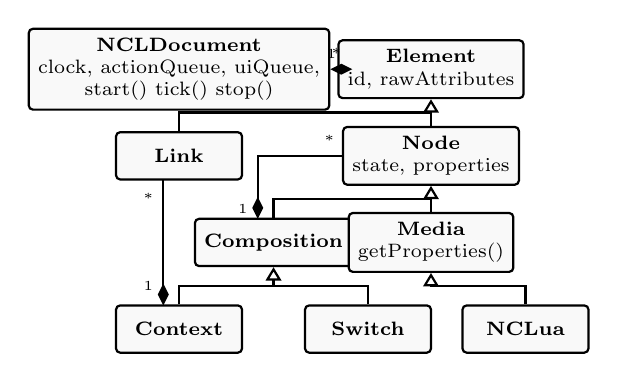
\begin{tikzpicture}[
      classbox/.style={draw, rectangle, rounded corners=1.5pt, minimum width=1.6cm, minimum height=0.6cm, align=center, fill=gray!5, thick, font=\scriptsize}
    ]
    \node [classbox] (ncldoc) at (-2.2, 2.0) {\textbf{NCLDocument} \\ clock, actionQueue, uiQueue, \\ start() tick() stop()};
    \node [classbox] (element) at (1.0, 2.0) {\textbf{Element} \\ id, rawAttributes};
    \node [classbox] (link) at (-2.2, 0.9) {\textbf{Link}};
    \node [classbox] (node) at (1.0, 0.9) {\textbf{Node} \\ state, properties};
    \node [classbox] (composition) at (-1.0, -0.2) {\textbf{Composition}};
    \node [classbox] (media) at (1.0, -0.2) {\textbf{Media} \\ getProperties()};
    \node [classbox] (context) at (-2.2, -1.3) {\textbf{Context}};
    \node [classbox] (switch) at (0.2, -1.3) {\textbf{Switch}};
    \node [classbox] (nclua) at (2.2, -1.3) {\textbf{NCLua}};

    \draw [thick, -{Triangle[open]}] (node.north) -- (element.south);
    \draw [thick] (link.north) |- (1.0, 1.45);

    \draw [thick, -{Triangle[open]}] (media.north) -- (node.south);
    \draw [thick] (composition.north) |- (1.0, 0.35);

    \draw [thick, -{Triangle[open]}] (context.north) |- (-1.0, -0.75) -- (composition.south);
    \draw [thick] (switch.north) |- (-1.0, -0.75);
    \draw [thick, -{Triangle[open]}] (nclua.north) |- (1.0, -0.75) -- (media.south);

    \draw [thick, {Diamond[fill=black]}-] (ncldoc.east) -- node[above, pos=0.15, font=\tiny] {1} node[above, pos=0.85, font=\tiny] {*} (element.west);
    \draw [thick, {Diamond[fill=black]}-] (-1.2, 0.1) -- node[left, pos=0.15, font=\tiny] {1} (-1.2, 0.9) -- node[above, pos=0.85, font=\tiny] {*} (node.west);
    \draw [thick, {Diamond[fill=black]}-] (-2.4, -1.0) -- node[left, pos=0.15, font=\tiny] {1} node[left, pos=0.85, font=\tiny] {*} (-2.4, 0.6);
  \end{tikzpicture}
  \caption{\texttt{gingaf} NCL \texttt{DOM}}
  \label{fig:elem_tree}
\end{figure}

\texttt{tick()} function advances an internal virtual clock by the given millisecond increment rather than relying on system time. This clock can be driven manually for testing or automatically by a Flutter periodic timer in a presentation environment. Decoupling time from the renderer enables high-speed headless testing: synchronization scenarios can be validated in-memory using inline XML strings, with no overhead from rendering windows, graphics libraries, or AV decoders.

On each call, \texttt{tick()} drains two queues. The \texttt{ActionQueue} collects transitions and link executions generated during state changes; these are drained deterministically in XML document definition order to ensure consistent execution behavior. The \texttt{UIQueue} serves communication across the component boundary: before the tick, the NCL UI component writes entries reporting that a media presentation has ended, which the engine processes to propagate any triggered links; after the tick, the engine writes entries indicating which \texttt{Media} nodes changed visual properties, so the NCL UI component can update rendering accordingly.

Decoupling the execution from the renderer enables high-speed, headless testing. Synchronization scenarios can be validated in memory using XML strings, completely removing the overhead of rendering windows, loading graphics libraries, or initializing native audio/video decoders. An example of the execution log produced during headless execution is shown in Listing~\ref{lst:logs}.

\begin{lstlisting}[caption={Log from headless execution of \texttt{video.ncl}}, basicstyle=\scriptsize\ttfamily, frame=single, breaklines=true, aboveskip=1mm, belowskip=1mm, captionpos=b, numbers=left, label={lst:logs}]
> dart run ncldoc/lib/main.dart ginga/examples/video.ncl
[ncldoc_cli] Executing ginga/examples/video.ncl in headless mode
[Clock: 0.0s] NCLDocument will start
[Clock: 0.0s] Node "body": sleeping->occurring
[Clock: 0.0s] Node "video": sleeping->occurring
[ncldoc_cli] perform 1 ticks per second indefinitely
[Clock: 0.0s] tickIndefinitely (1 ticks per/s)
[Clock: 1.0s] Tick
[Clock: 2.0s] Node "video" (area a1): sleeping->occurring
[Clock: 2.0s] Node "green_bg": sleeping->occurring
[Clock: 2.0s] Tick
[Clock: 3.0s] Tick
[Clock: 4.0s] Node "video" (area a1): occurring -> sleeping
[Clock: 4.0s] Node "green_bg": occurring -> sleeping
[Clock: 4.0s] Node "red_bg": sleeping->occurring
\end{lstlisting}

\subsection{\projectname{} NCL UI}
\label{sec:nclui}

The \projectname{} NCL UI component is responsible for visual presentation. \texttt{NCLWidget} drives the engine by calling \texttt{tick()} on \texttt{NCLDocument} (arrow~2 in Figure~\ref{fig:arch}) and delegates rendering to \texttt{NCLMediaState}, which reads the current visual properties of each \texttt{Media} node directly from the NCL logic component (arrow~5). The interface is composed of a root \texttt{Ginga} widget that utilizes a Flutter \texttt{Stack} to layout widgets. A background audio/video widget (\texttt{main\_av\_widget}) is placed at the bottom, and the active media elements are rendered on top within the NCL presentation surface. The \texttt{WidgetFactory} maps NCL elements to native Flutter widgets.

Currently implemented widgets include: \texttt{ImageWidget}: Displays images and handles image format caching; \texttt{AVWidget}: Renders native video/audio playback, supporting state tracking; and \texttt{TextWidget}: Renders formatted text blocks using bounds properties. Each widget extends \texttt{BaseWidget}, which maps NCL layout properties (like \texttt{left}, \texttt{top}, \texttt{width}, \texttt{height}, and \texttt{background}) to Flutter layout parameters (\texttt{Positioned} and \texttt{BoxDecoration}).

A key design aspect of \projectname{} is that \texttt{NCLWidget} holds an instance of \texttt{NCLDocument} and registers a Flutter periodic timer that periodically calls \texttt{doc.tick()} to advance the virtual clock. When a media widget experiences a state change (for example, when an \texttt{AVWidget} reaches the end of its video file), the widget notifies the \texttt{NCLWidget} via the UI Queue. The application then retrieves the corresponding \texttt{Media} node from the document and triggers its transition event, allowing the headless execution engine to run link conditions and propagate state changes back to the widgets. This ensures a clean separation of concerns: widgets only worry about rendering and local lifecycle events, while the engine handles the declarative NCL coordination logic.

\section{Results}

To show the correctness and multiplatform execution capabilities of \projectname{}, we execute the sample NCL application (\texttt{video.ncl}) described in Section~\ref{sec:background}. As a result, Figure~\ref{fig:multiplatform} presents the execution of this application across three different environments: Windows, Android, and Web. Additionally, the temporal execution screenshots are shown in Figure~\ref{fig:running} and the corresponding logs are provided in Listing~\ref{lst:logs}.

\begin{figure}[ht]
  \centering
  \Description{Screenshots of \texttt{video.ncl} across Windows, Android, and Web browsers.}
  \begin{subfigure}{0.32\linewidth}
    \centering
    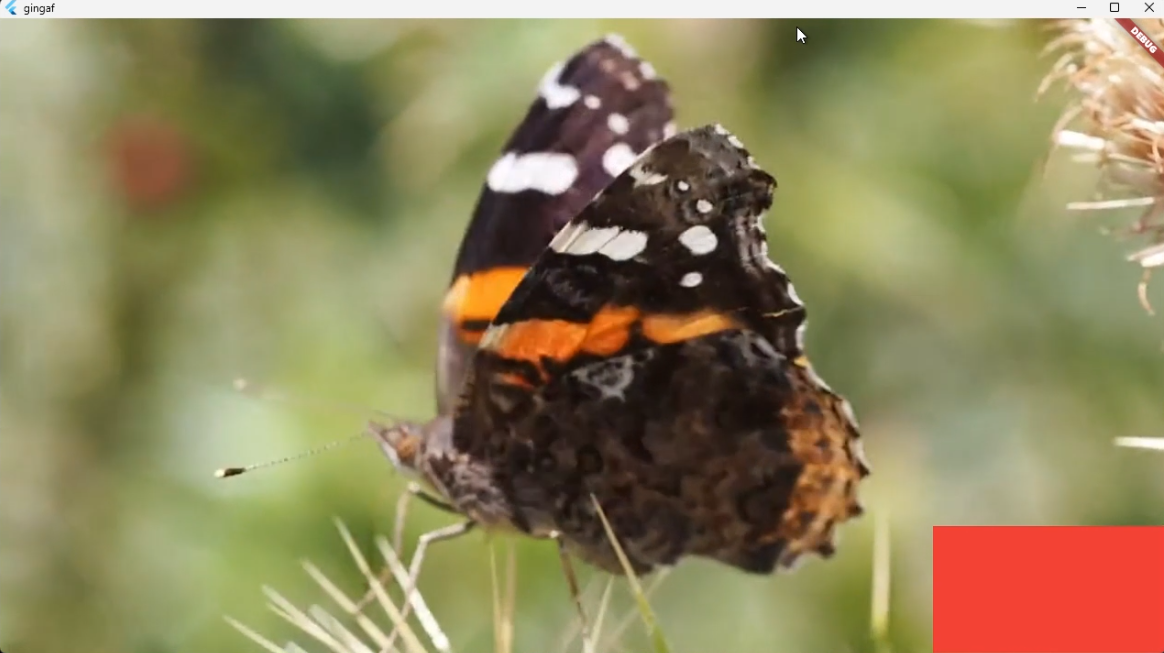
\includegraphics[width=\linewidth]{assets/app_clock4.png}
    \caption{Windows.}
    \label{fig:res_windows}
  \end{subfigure}%
  \hfill%
  \begin{subfigure}{0.32\linewidth}
    \centering
    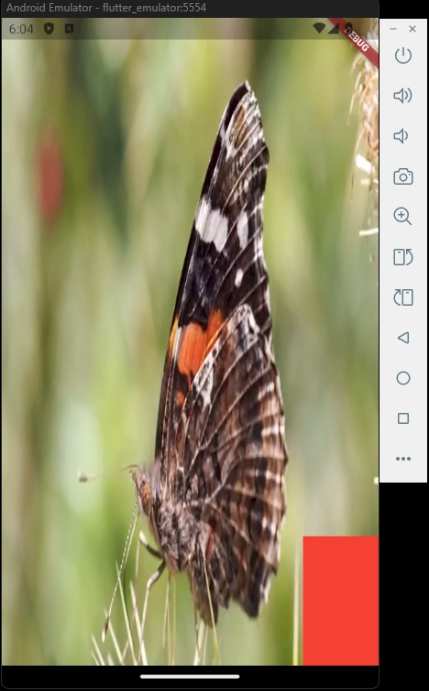
\includegraphics[height=2.8cm, keepaspectratio]{assets/android.png}
    \caption{Android.}
    \label{fig:res_android}
  \end{subfigure}%
  \hfill%
  \begin{subfigure}{0.32\linewidth}
    \centering
    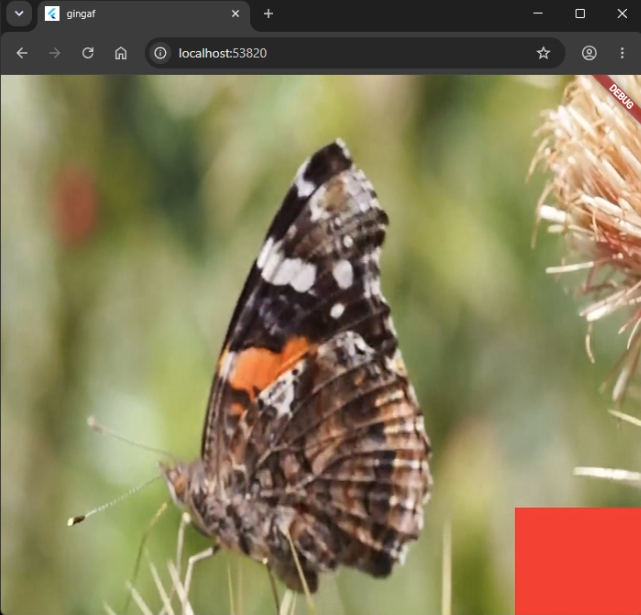
\includegraphics[width=\linewidth]{assets/web.png}
    \caption{Web.}
    \label{fig:res_web}
  \end{subfigure}
  \caption{\texttt{video.ncl} running on Windows, Android, and Web.}
  \label{fig:multiplatform}
\end{figure}

The reliability of the codebase is maintained through an automated test suite. The \texttt{ncl\_doc} logic package contains 64 unit tests validating the parser, XML parsing rules, virtual clock progression, and deterministic link execution. The \texttt{gingaf} presentation package contains 14 tests verifying widget rendering, layout constraint resolution, focus state transitions, and integration with the NCL execution engine. All tests run in milliseconds due to the headless execution capabilities of the engine.

To replicate our results, we guide the reader to execute the commands below:

\begin{lstlisting}[language=bash, basicstyle=\scriptsize\ttfamily, frame=single, breaklines=true]
$ git clone -b v0.1.0 https://github.com/ginga-org-br/gingaf
$ cd gingaf/ncldoc
$ make deps
# Headless execution of video.ncl
$ dart lib/main.dart ../ginga/examples/video.ncl
# UI execution of video.ncl
$ cd ../ginga
$ make deps # See SETUP.md for environment configuration
$ flutter run -d <chrome,windows,emulator-XXXX> --dart-define="APP=examples/video.ncl"
\end{lstlisting}

\section{Final Remarks}

\projectname{} demonstrates that decoupling the NCL logic component from the NCL UI component provides a flexible, testable, and highly portable solution for executing NCL digital television applications. The NCL logic component, implemented as \texttt{ncl\_doc}, directly addresses \textbf{P2 (Lack of NCL Debugging Features)}: it runs fully in-memory with no rendering dependency, enabling deterministic unit testing of NCL synchronization logic. The NCL UI component, built on Flutter, directly addresses \textbf{P1 (Lack of Accessible NCL Development Environment)}: it compiles to Windows, mobile, and web from a single codebase, removing the need for specialized hardware or platform-specific setups.

Next steps include the development of a web-based NCL playground that integrates debugging features to allow developers to run and step through NCL applications directly in the browser without any local installation, closing the accessibility gap for NCL developers and researchers.

\bibliographystyle{ACM-Reference-Format}
\bibliography{references}

\appendix

\end{document}